\documentclass[]{article}
\usepackage{array}
\usepackage[table]{xcolor}
\usepackage{graphicx}
\newcolumntype{M}[1]{>{\centering\arraybackslash}m{#1}}
\usepackage{graphicx}
\usepackage{amsmath}
\usepackage{float}
\restylefloat{table}
\renewcommand{\arraystretch}{1.2}

\usepackage{hyperref}

%opening
\title{Big Data Mining - Assignment}
\author{Dimitrios Vogiatzis}
\author{
	Dimitrios Vogiatzis\\
	\texttt{CS2.18.0004}
	\and
	Victor Giannakouris\\
	\texttt{CS3.18.0002}
}

\begin{document}
\date{}
\maketitle

\section{Abstract}
In this report we describe in detail the techniques that we used in the assignment of the Big Data Mining course. In summary, given an news input dataset the main goals of this assignment were to generate a Wordcloud for each possible category, duplicate detection with respect to the cosine distance metric, the implementation and evaluation of several state-of-the-art classification algorithms, as well as a custom architecture that overperforms the aforementioned state-of-the-art algorithms in terms of a number of evaluation metrics. Through experimental evaluation we showcase that our architecture achieves better performance for all of the evaluation metrics that we have used, including accuracy, precision, recall, ROC and F-Measure.
\section{Introduction}
\subsection{Goals}
The goal of this assignment is the development of a system that will meet all the requirements by implementing modules for the following: 1. Generation of a Wordcloud for each of the available news categories, 2. Detection of articles with high degree of similarity between them (duplicate detection), 3. The implementation and evaluation of several state-of-the-art classification algorithms and 4. The development of a custom architecture that will outperform the algorithms defined in 3.
\subsection{Installation}
In this section we describe the steps required for installing and running our system. For these steps, an installation of \emph{virtualenv}\footnote{https://virtualenv.pypa.io/en/latest/} is required.
\begin{enumerate}
	\item Clone the repository:\\
	\texttt{git clone git@github.com:dcvogi/big-data-uoa.git}
	\item Create a virtual environment using \emph{virtualenv}:\\
	\texttt{virtualenv .venv -p /usr/bin/python2.7}
	\item Load the virtual environment:\\ 
	\texttt{source .venv/bin/active}
	\item Install the requirements defined in \emph{src/requirements.txt}:\\
	\texttt{pip install -r requirements.txt}
	\item Run \emph{main.py}:\\
	\texttt{python main.py}
\end{enumerate}
After step 5 is completed, the results including \emph{duplicatePairs.csv}, \emph{EvaluationMetric\_10fold.csv} and all the .png Wordcloud images will be generated inside \emph{results} folder.
\section{Implementation}
\subsection{Wordcloud}
In this task, we generated the Wordcloud for each of the input set categories. Wordcloud generation is a quite simple task. After a single pass to each document of each category the word frequencies for each category are generated. The Wordcloud of each frequency is generated with respect to these frequencies, were the size of a word image in the final word cloud results directly from its frequency. That is, the size of a word $a$ will be larger that the size of a word $b$ if $a$ has a higher frequency. For this task we used the WordCloud\footnote{https://amueller.github.io/word\_cloud/} python package.
\subsection{Duplicates Detection}
This section is responsible for describing in detail the methodology used in order to detect duplicate documents.
\subsubsection{Vectorizer}
In order to compute the similarity of the documents, we must first  produce the term vectors for each document of the dataset (test set). To do that we used TfidfVectorizer from Python sklearn library. TfidfVectorizer converts a collection of raw documents to a matrix of TF-IDF features. TF-IDF, short for term frequency-inverse document frequency, is a numerical statistic that is intended to reflect how important a word is to a document in a collection or corpus. \cite{rajaraman2011datamining}
\subsubsection{Similarity detection}
At this stage and after we produced the term vectors with TfidfVectorizer, we compute the cosine similarity between the  vectors of each document versus the others, ending up with a $n \times n$  matrix where the value of the pair $\imath, \jmath$ corresponds to the cosine of the angle between them (similarity). In order to avoid double-checking the same pairs, we traverse the upper triangular of the matrix keeping only the pairs with similarity greater than the input threshold $\theta$. 
\subsection{Classification Implementation}
In this section we describe in detail the libraries that we used in order to implement the required classification algorithms, vectorizers, as well as dimensionality reduction modules.
%
\subsubsection{Vectorizers}
Two vectorizers were used for the assignment’s purposes, that is, a bag-of-words (BOW) model and the Word2Vec (W2V) model.
\\
\textbf{Bag-of-Words.} The bag-of-words\cite{BoW} model is one of the simplest approaches used in text mining. A document is represented as a $n$-sized vector, where $n$ the size of the dictionary. An element at the position $i$ of a vector $X$ represents the frequency of the $i^{th}$ word of the dictionary in the vector $X$, where $i$ denotes the word index. We used the \emph{CountVectorizer} instance of scikit-learn library for leveraging the Bag-of-Words model. Below there is a sample code snippet.
\begin{verbatim}
	from sklearn.feature_extraction.text import CountVectorizer
	
	input_docs = open("docs.txt").readlines()
	cv = CountVectorizer()
	cv.fit(input_docs)
\end{verbatim}
%
\textbf{Word2Vec.} Word2Vec\cite{mikolov2013distributed} is a more complex model. In summary, Word2Vec is a two-layer neural network trained to reconstruct linguistic contexts of words, which are also called \emph{word embeddings}\cite{WordEmbedding}. In this model each word is represented as a vector of numbers, in contrast with conventional models like TF-IDF where each word is represented as a single weight number. The main benefit of representing words as vectors is that different words with the same meaning will be close each other in the vector space, i.e. the word "king" will be close to the word "queen".

To implement Word2Vec we used the gensim\footnote{\url{https://radimrehurek.com/gensim/}} library. As aforementioned, Word2Vec converts each word into a vector of numbers and thus, each input document vector is transformed into a vector of word vectors. This vector of vectors form leads into compatibility issues, as far as scikit's classification models take as input only vectors of numbers. To resolve that, we implemented a custom vectorizer class that overrides the three basic vectorization methods, that is, \texttt{fit()}, \texttt{transform()} and \texttt{fit\_transform()}. The \texttt{fit()} method generates a Word2Vec model using the \texttt{from gensim.models import Word2Vec} class. The \texttt{transform()} takes as input a document in vector form. First, the document vector is being transformed into a vector of word vectors. Next, we generate an average vector, where each word vector is transformed into a mean value, resulting into a final document vector of means. Given an input vector $X$ as follows:
\begin{equation*}
		X=
	\begin{bmatrix}
	w_1\\
	w_2\\
	.\\
	.\\
	w_n
	\end{bmatrix} 
	\space
\end{equation*}
The $transform()$ method  can be defined by equation \ref{eq1} .
\begin{equation}
\label{eq1}
	transform(X) = mean(X) =
	\begin{bmatrix}
	mean(w_1) \\
	mean(w_2) \\

	. \\
	mean(w_n)
	\end{bmatrix} 
	=
	\begin{bmatrix}
	w_1' \\
    w_2' \\
	. \\
	. \\
	w_n'
	\end{bmatrix} 
\end{equation}

\subsection{Neural Network Architecture}
In order to achieve better performance than the algorithms described in subsection 3.3, we decided to proceed with changing both the classification algorithm and the vectorizer used both for experimentation and performance optimization.

\subsubsection{Vectorizer}
For this architecture we used Python's scikit-learn HashingVectorizer. HashingVectorizer applies a hashing function to term frequency counts in each document making it an efficient way of mapping terms to features. Even though using a hash function can lead to collisions (e.g. distinct tokens mapped to the same feature index), with HashingVectorizer this is rarely an issue as there is a parameter, \textit{n\_features}, that can be tweaked to avoid collisions. The parameter \textit{n\_features} refers to the number of features (columns) in the output matrices. In our tests we tried different values for \textit{n\_features} and after many tests we decided that with the given dataset, the most performing value was \textit{n\_features}=$2^{18}$ which is the recommended one for text classification problems.

\subsubsection{Classification Algorithm}
In the shake of experimentation we decided to implement a neural network for this task.
\subsection{Results}
In this section we describe in detail the results from our experimental evaluation, which consists of the generation of wordclouds, document duplicate detection and classification algorithm performance comparison.

\subsubsection{Wordcloud}
For each of the input set categories we generated the following wordclouds:

\begin{figure}[H]
\centering
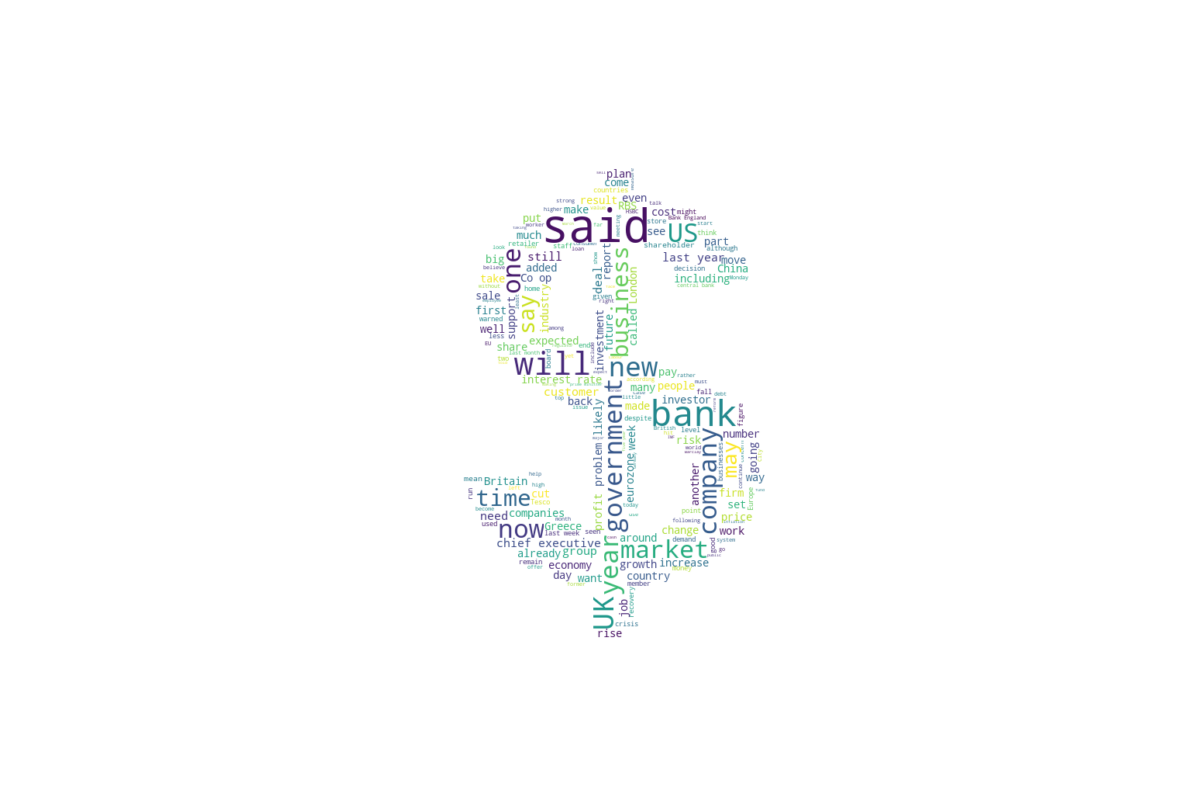
\includegraphics[scale=0.35]{images/Wordcloud_Business.png}
\caption{Business}
\end{figure}

\begin{figure}[H]
\centering
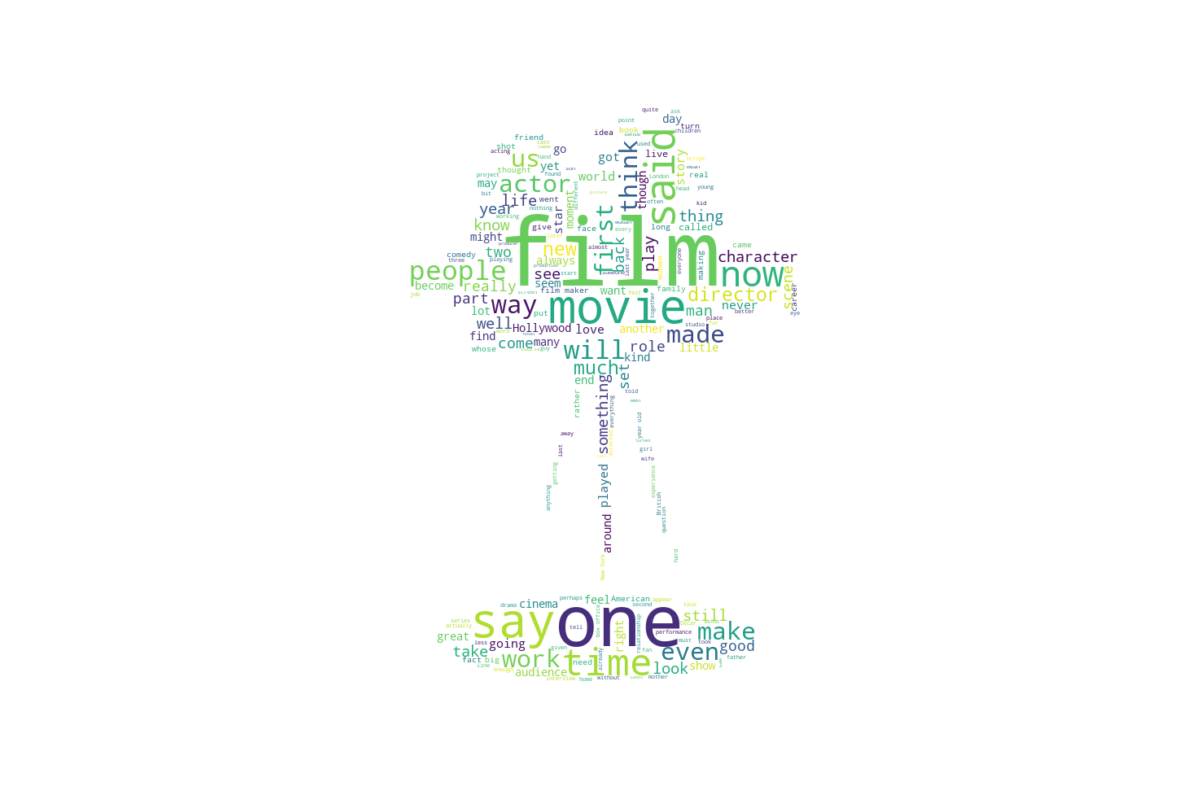
\includegraphics[scale=0.35]{images/Wordcloud_Film.png}
\caption{Film}
\end{figure}

\begin{figure}[H]
\centering
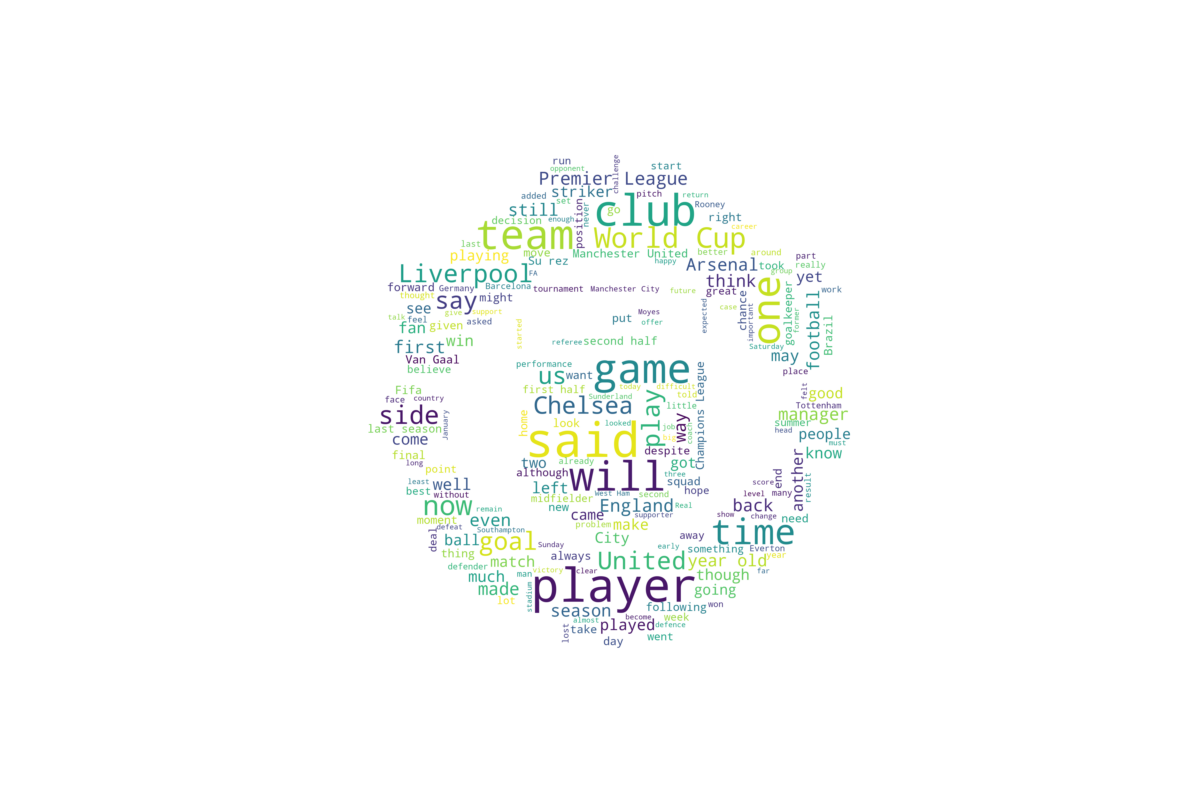
\includegraphics[scale=0.35]{images/Wordcloud_Football.png}
\caption{Football}
\end{figure}

\begin{figure}[H]
\centering
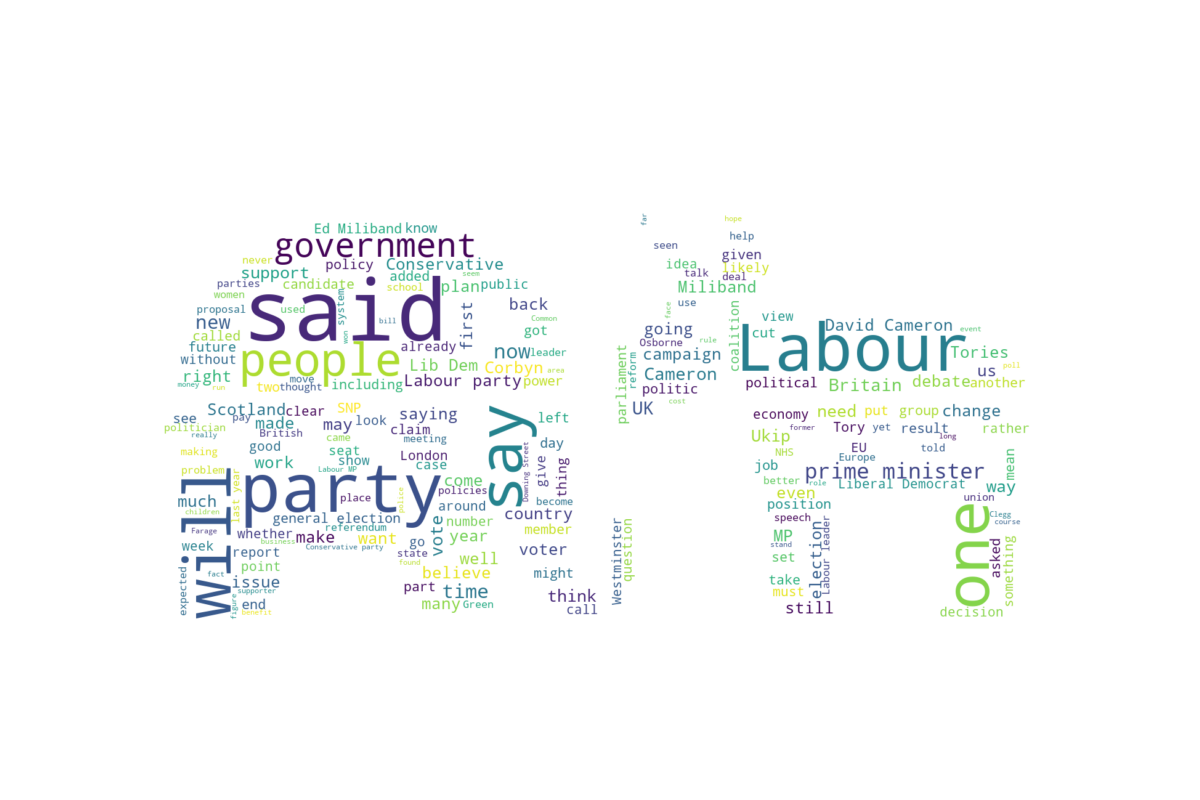
\includegraphics[scale=0.35]{images/Wordcloud_Politics.png}
\caption{Politics}
\end{figure}

\begin{figure}[H]
\centering
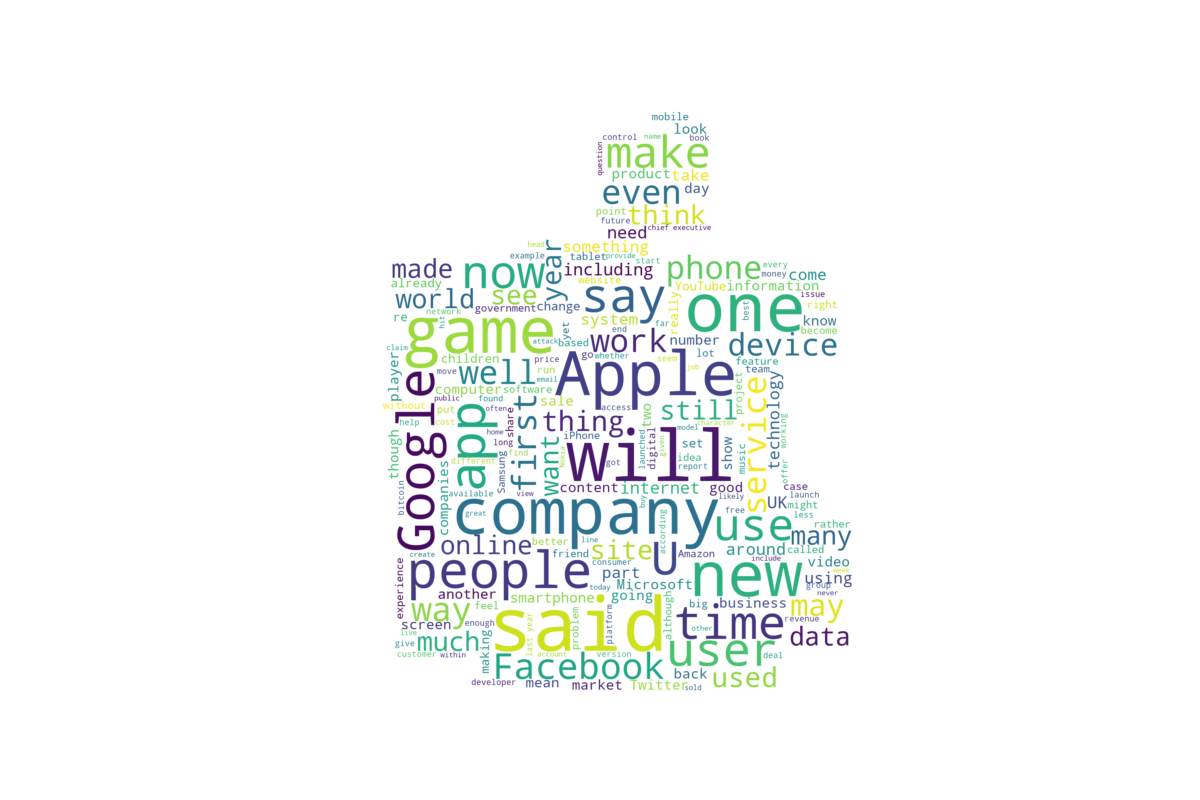
\includegraphics[scale=0.35]{images/Wordcloud_Technology.png}
\caption{Technology}
\end{figure}
\newpage
\subsubsection{Duplicates Detection}
As requested, the given source code accepts an input parameter $\theta$ as the similarity threshold. To export the results, we used $\theta = 0.7$ and based on this threshold, an output file (duplicatePairs.csv) is generated including all the document pairs with cosine similarity $>= 0.7$. Below is a small sample of the output file: \newline

\begin{tabular}{ |M{3cm}|M{3cm}|M{3cm}|  }
    \hline
    \rowcolor{lightgray!60}
    \multicolumn{3}{|c|}{duplicatePairs.csv} \\
    \hline 
    \rowcolor{lightgray!40}
    Document\_ID1& Document\_ID2 & Similarity \\
    \hline
    10802 & 10213 & 0.7104 \\
    10802 & 13991 & 0.7073 \\
    6727 & 1015 & 0.7134 \\
    ... & ... & ... \\
    7811 & 11213 & 0.7150 \\
    14607 & 11213 & 0.7661 \\
    \hline
\end{tabular}

\subsubsection{Classification Algorithms}
Below you can find the evaluation metric table which holds the performance of each classification algorithm implemented:

\begin{table}[H]
    \hspace{-50pt}
    \begin{tabular}{|>{\columncolor{lightgray!40}}l|l|l|l|l|l|l|l|l|l|}
        \hline
        \rowcolor{lightgray!40}
        Measure &  SVM(BoW) &  RF(BoW)  & SVM(SVD) & RF(SVD) & SVM(W2V) & RF(W2V)  & NN\\ \hline
        Accuracy & 0.935 & 0.927 & 0.931 & 0.929 & 0.935 & 0.889 & 0.964 \\ \hline
        Precision & 0.932 & 0.925 & 0.928 & 0.927 & 0.930 & 0.885 & 0.962 \\ \hline
        Recall & 0.929 & 0.916 & 0.925 & 0.920 & 0.929 & 0.878 & 0.961 \\ \hline
        F-Measure & 0.930 & 0.920 & 0.926 & 0.923 & 0.929 & 0.881 & 0.962 \\ \hline
        AUC & 0.956 & 0.949 & 0.954 & 0.951 & 0.956 & 0.925 & 0.976 \\ \hline
    \end{tabular}
    \caption{EvaluationMetric\_10fold.csv}
\end{table}
\noindent
Testing the performance of the MLP, using the token vectors from \textit{HashingVectorizer} we managed to achieve a performance increase over the methods used in subsection 3.3 as shown above, in the evaluation metric table (EvaluationMetric\_10fold.csv). The performance of this architecture was consistently better as there were multiple experiments with different seeds and inputs. With our custom architecture (Neural Network) we generated an output file (testSet\_categories.csv) which holds all the predicted categories for each document of the test set. The format of the output file is shown in the sample below:\\
\begin{table}[H]
\centering
\begin{tabular}{ |M{5cm}|M{5cm}|  }
    \hline
    \rowcolor{lightgray!60}
    \multicolumn{2}{|c|}{testSet\_categories.csv} \\
    \hline 
    \rowcolor{lightgray!40}
    Test\_Document\_ID & Predicted\_Category \\
    \hline
    2 & Politics \\
    10 & Technology \\
    25 & Technology \\
    ... & ... \\
    15332 & Football \\
    15333 & Football \\
    \hline
\end{tabular}
\end{table}



\bibliographystyle{unsrt}
\bibliography{report}

\end{document}